\documentclass{standalone}
\usepackage{tikz}
\usepackage{ctex,siunitx}
\setCJKmainfont{Noto Serif CJK SC}
\usepackage{tkz-euclide}
\usepackage{amsmath}
\usepackage{wasysym}
\usetikzlibrary{patterns, calc}
\usetikzlibrary {decorations.pathmorphing, decorations.pathreplacing, decorations.shapes,}
\begin{document}
\small
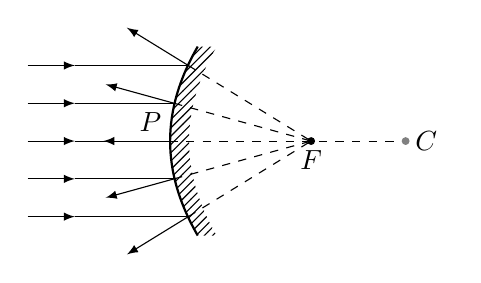
\begin{tikzpicture}[>=latex,scale=1.2]
  \useasboundingbox(-4,1.2)rectangle(0.5,-1.2);
  \fill [pattern=north east lines] (-2,-1)--(-2.2,-1) to [bend left=30] (-2.2,1) --(-2,1) to [bend left=-30]
  (-2,-1);
  \draw [thick](-2.2,1) to [bend left=-30] (-2.2,-1);
  \foreach \x in {-.8,-.4,0,...,.8}
      {
          \draw[->] (-4,\x)--(-3.5,\x);
      }    
  \draw(-3.5,-.8)--(-2.3,-.8);
  \draw(-3.5,-.4)--(-2.45,-.4);
  \draw(-3.5,.4)--(-2.45,.4);
  \draw(-3.5,.8)--(-2.3,.8);
  \draw(-3.5,0)--(-2.5,0);  
  \draw[->](-2.5,0)--(-3.2,0);
  \draw[dashed] (-2.5,0)--(-1,0)node [below]{$F$}--(0,0)node [right]{$C$};
  \draw [dashed](-2.3,-.8)--(-1,0);
  \draw [dashed](-2.45,-.4)--(-1,0);
  \draw [dashed](-2.45,.4)--(-1,0);
  \draw [dashed](-2.3,.8)--(-1,0);
  \draw [->](-2.3,-.8)--(-2.95,-1.2);
  \draw [->](-2.45,-.4)--(-6.35/2,-.6);
  \draw [->](-2.45,.4)--(-6.35/2,.6);
  \draw [->](-2.3,.8)--(-2.95,1.2);
  \node at (-2.7,0)[above]{$P$};
  \draw (-1,0)[ fill=black] circle (1pt);
  \draw (0,0)[gray,fill=gray] circle (1pt);
\end{tikzpicture}
\end{document}